\documentclass[extrafontsizes,60pt,twocolumn]{memoir}
\setstocksize{48in}{96in}
\settrimmedsize{48in}{96in}{*}
\setlrmarginsandblock{1in}{1in}{*}
\setulmarginsandblock{1.4in}{20mm}{*}

\usepackage[utf8]{inputenc} % allow utf-8 input
\usepackage[T1]{fontenc}    % use 8-bit T1 fonts
\usepackage[svgnames,table]{xcolor}
\usepackage[none]{hyphenat}
\usepackage{graphicx}
\usepackage{array}
\usepackage[font=small,labelfont=bf]{caption}
\usepackage{amsfonts, amsmath, amsthm, amssymb}
\usepackage{adjustbox}
\usepackage[absolute,overlay]{textpos}
\usepackage{multirow}
\usepackage{titlesec}
\usepackage{cuted}
\usepackage[inline]{enumitem}
\usepackage{url}
\usepackage{tikz,pgfplots,pgfplotstable}
\usepackage[most]{tcolorbox}
\usepackage[charter]{mathdesign}
\usepackage{subcaption}
\usepackage{multirow}
\usetikzlibrary{arrows.meta}
\captionsetup{labelformat=empty}
\graphicspath{{figures/}}
\renewcommand{\chapter}[2]{}

% for confusion matrix
\newcommand{\ApplyGradient}[1]{%
  \pgfmathsetmacro{\PercentColor}{(#1-0)/63.88}%
  \pgfmathsetmacro{\PercentInverse}{ifthenelse(\PercentColor > 70, 0, 100)}%
  %\textcolor{black!\PercentColor}{#1}
  \edef\x{\noexpand\cellcolor{red!\PercentColor}}\x\textcolor{black!\PercentInverse}{#1}%
}
\newcolumntype{R}{>{\collectcell\ApplyGradient}{c}<{\endcollectcell}}

\begin{document}

\setlength{\columnseprule}{1pt}

\begin{strip}
  \begin{center}
  \scalebox{1.75}{
    \HUGE\textbf{Syntactic Interchangeability in Word Embedding Models}}
  \end{center}
  \begin{center}
  \begin{minipage}[b]{.9\linewidth}
    \centering
    \begin{minipage}{.8\linewidth}
      \HUGE\textbf{Daniel Hershcovich} \& \textbf{Assaf Toledo} \& \textbf{Alon Halfon} \& \textbf{Noam Slonim}
    \end{minipage}
    \hfill
    \begin{minipage}{.15\linewidth}
      \HUGE\textbf{IBM Research}
    \end{minipage}
    
    \vspace{.5in}
    \titlespacing*{\section}{0pt}{8mm}{.5in}
    \begin{adjustbox}{margin=.5in,frame,minipage=\textwidth,center,color=purple,cfbox=green}
      \centering\huge
      Do word embeddings capture part-of-speech? \\
      Explaining the effect of context window size on word similarity evaluation.
    \end{adjustbox}
  \end{minipage}
  \end{center}
\end{strip}

%----------------------------------------------------------------------------------------

\section*{Word Similarity and Relatedness Benchmarks}


    \begin{figure}[h]
        \begin{subfigure}[c]{.2\columnwidth}
          300-dimensional fastText embeddings trained on Wikipedia with the CBOW and SGNS algorithms.
          
          \vspace{1in}
          Measuring cosine similarity between words in each benchmark pair.
        \end{subfigure}
        \hspace{1in}
        \begin{subfigure}[c]{.35\columnwidth}
        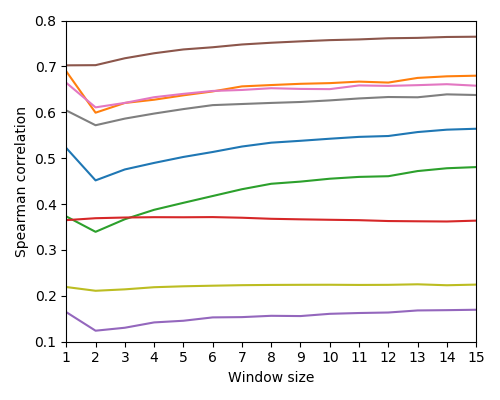
\includegraphics[width=\columnwidth]{similarities_fasttext_enwiki-20170501-clean_cbow-300d-min500_eval.png}
        \caption{CBOW}
        \end{subfigure}
        \hfill
        \begin{subfigure}[c]{.35\columnwidth}
        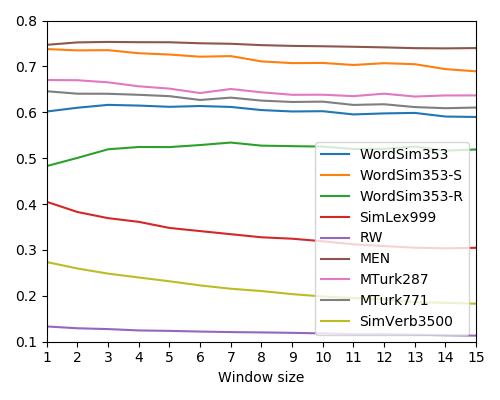
\includegraphics[width=\columnwidth]{similarities_fasttext_enwiki-20170501-clean_skipgram-300d-min500_eval.png}
        \caption{SGNS}
        \end{subfigure}
    \end{figure}
    
\hrule

\section*{Interchangeability Enrichment in Benchmarks and in Word Embedding Models}

    \begin{table}[h]
    \def\arraystretch{1.6}
    \setlength\tabcolsep{.1in}
    \begin{tabular}{m{.23\columnwidth}}
      Words are approximately \textit{\textbf{syntactically interchangeable}}
      if they have the same POS (part-of-speech).
    \end{tabular}
    \hspace{1in}
    \scalebox{.6}{
    \begin{tabular}{l|c||cc||cc|cc|c}
    && \multicolumn{2}{c||}{\textbf{$\Delta \mathtt{win}=2\to 15 (\%)$}}
    & \multicolumn{2}{c|}{\textbf{$\#$ Related}} & \multicolumn{2}{c|}{\textbf{$\#$ Unrelated}} \\
    \textbf{Benchmark} & \textbf{Size} & \textbf{CBOW} & \textbf{SGNS}
    & \textbf{All} & \textbf{Same-POS} & \textbf{All} & \textbf{Same-POS} & \textbf{p-value} \\
    \hline
    WordSim353 & 353 & 24 & -3 & 122 & 107 & 53 & 40 & 0.038 \\
    WordSim353-S & 203 & 13 & -6 & 60 & 53 & 53 & 40 & 0.061 \\
    WordSim353-R & 252 & 42 & 4 & 104 & 89 & 39 & 31 & 0.26 \\
    SimLex999 & 999 & -1 & -20 & 234 & 199 & 334 & 295 & 0.897 \\
    RW & 2034 & 37 & -12 & 944 & 555 & 262 & 144 & 0.149 \\
    MEN & 3000 & 9 & -2 & 791 & 564 & 781 & 439 & $3\cdot10^{-10}$ \\
    MTurk287 & 287 & 8 & -5 & 49 & 39 & 119 & 68 & 0.004 \\
    MTurk771 & 771 & 12 & -5 & 204 & 153 & 200 & 146 & 0.365 \\
    SimVerb3500 & 3500 & 6 & -30 & 633 & 265 & 1217 & 566 & 0.974
    \end{tabular}}
    \hspace{1in}
    \scalebox{.9}{
    \begin{tabular}{l|ccc|ccc|ccc}
    {\textbf{Algo-}} & \multicolumn{3}{c|}{\textbf{NOUN}} & \multicolumn{3}{c|}{\textbf{ADJ}} & \multicolumn{3}{c}{\textbf{VERB}} \\
    {\textbf{rithm}} & 1 & 15 & r & 1 & 15 & r & 1 & 15 & r \\
    \hline
    &&&&&&\\
    CBOW & 79 & 70 & -0.96 & 72 & 48 & -0.93 & 55 & 41 & -0.91 \\
    &&&&&&\\
    SGNS & 78 & 66 & -0.95 & 66 & 39 & -0.94 & 51 & 41 & -0.92 
    \end{tabular}}
    \end{table}
    
\section*{Number of Neighbors per POS}
    
    \begin{figure}[h]
        \begin{subfigure}[c]{.2\columnwidth}
        Context window size is negatively correlated with interchangeability.
        \vspace{5in}
        
        \hfill
        
\includegraphics[width=.9\textwidth]{qr.png}
        \end{subfigure}
        \hspace{1in}
        \begin{subfigure}[c]{.35\columnwidth}
        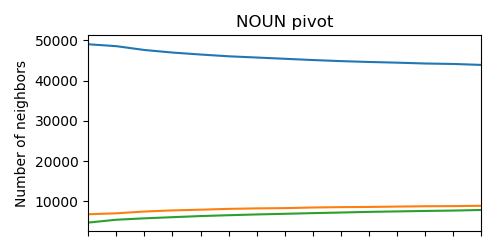
\includegraphics[width=\columnwidth]{NOUN_nn_100_fasttext_enwiki-20170501-clean_cbow-300d-min500_pos.png}
        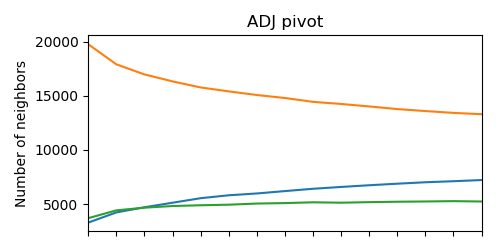
\includegraphics[width=\columnwidth]{ADJ_nn_100_fasttext_enwiki-20170501-clean_cbow-300d-min500_pos.png}
        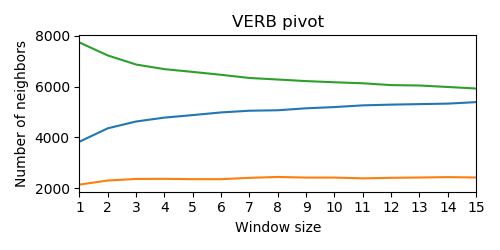
\includegraphics[width=\columnwidth]{VERB_nn_100_fasttext_enwiki-20170501-clean_cbow-300d-min500_pos.png}
        \caption{CBOW}
        \end{subfigure}
        \hfill
        \begin{subfigure}[c]{.35\columnwidth}
        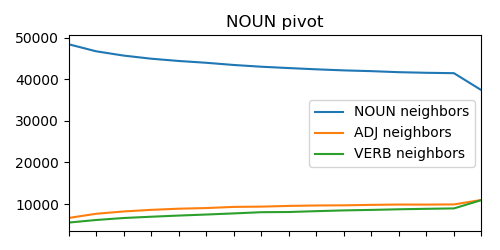
\includegraphics[width=\columnwidth]{NOUN_nn_100_fasttext_enwiki-20170501-clean_skipgram-300d-min500_pos.png}
        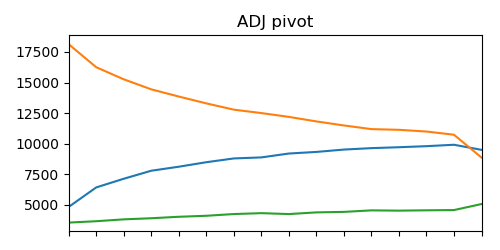
\includegraphics[width=\columnwidth]{ADJ_nn_100_fasttext_enwiki-20170501-clean_skipgram-300d-min500_pos.png}
        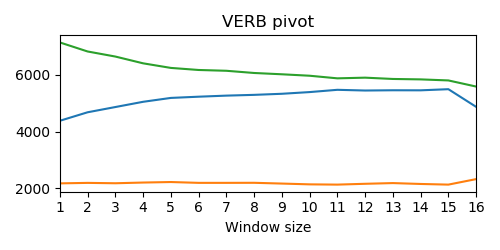
\includegraphics[width=\columnwidth]{VERB_nn_100_fasttext_enwiki-20170501-clean_skipgram-300d-min500_pos.png}
        \caption{SGNS}
        \end{subfigure}
    \end{figure}

\vfill\hfill
\url{https://github.com/danielhers/interchangeability}


\begin{minipage}{.42\columnwidth}
\color{DarkSlateGray}
\tiny
\setlength\bibitemsep{0pt}
\bibliographystyle{plain}
\bibliography{references}
\end{minipage}
\hspace{.3in}
\begin{minipage}{.475\columnwidth}
\color{Black}
\end{minipage}


\end{document}
